\chapter{فيزيولوجيا الكلية وتنظيم الأسمولية}\label{ch:b3:renal-osmoregulation}

ترشّح كليتاك مئة وثمانين لترًا من البلازما في اليوم --- أي
حجم دمك كله كل نصف ساعة --- وتعيدان كل ذلك إلا لترًا ونصف
لتر، وقد أخرجتا البولة، وضبطتا الملح والحمض والماء إلى حدود
واحد في المئة مما يحتاج إليه الجسم، وحفظتا كل غرام من
الغلوكوز. وجرذ الكنغر في الصحراء لا يشرب البتة: فهو يعيش على
الماء الذي يصنعه استقلابه من بذور جافة ويطرح بولًا أغلظ من
ماء البحر خمس مرات. وسمكة بحرية تشرب باستمرار وتضخ الملح إلى
الخارج عبر خياشيمها؛ وسمكة عذبة لا تشرب أبدًا وتضخ الملح إلى
الداخل. والمسألة التي تحلها كلها واحدة: أن تبقي تركيب السائل
حول الخلايا ثابتًا بينما يشوّشه الأكل والشرب والتنفس، وأن
تتخلص من النتروجين من غير أن تتخلص من ماء أكثر مما ينبغي.
ويتناول هذا الفصل كلية الثدييات مثالًا محلولًا --- الرشح،
وحساب التصفية، وحيلة التيار المعاكس التي تغلّظ البول،
والهرمونات التي تضبط الأقراص --- ثم مدى الحلول عبر الحيوانات.

\section{المسألة}

\begin{definition}[تنظيم الأسمولية]\label{def:b3:renal-osmoregulation:problem}
\index{أسمولية}\index{ضغط حلولي}\index{سائل خارج خلوي}\index{مطابق أسموزي}\index{منظِّم أسموزي}
\emph{أسمولية} محلول هي تركيزه الكلي من الجسيمات المنحلّة
(بالأسمولات في اللتر)؛ وهي تحدد \emph{الضغط الحلولي}،
$\Pi = cRT$ للمحاليل المخففة، الذي يسوق الماء عبر أي غشاء
يمرر الماء لا المذاب. وسوائل جسم الثديي عند نحو
\qty{300}{mOsm/L} --- و\qty{40}{\%} من كتلة الجسم داخل
الخلايا، و\qty{20}{\%} خارجها، وهو \emph{السائل خارج الخلوي}
الذي رُبعه بلازما --- وتنتفخ الخلايا أو تنكمش في ثوانٍ إذا
تغيّر الخارج، إذ تمرر أغشيتها الماء بحرية. و\emph{المطابق
الأسموزي} (ومنه معظم اللافقاريات البحرية، والقروش) يبقي
سوائله عند أسمولية البحر ولا ينظم إلا تركيبها؛ و\emph{المنظِّم
الأسموزي} (ومنه الفقاريات، والحشرات، وحيوانات الماء العذب)
يبقي أسموليته ثابتة في مواجهة البيئة، وهو ما يكلف طاقة
تتناسب مع التدرج. والمهمة الثانية، المقترنة بالأولى، هي
التخلص من نتروجين هدم البروتين: إما \emph{نشادرًا} في ماء
وفير (الأسماك)، وإما \emph{بولةً} منحلّة غير سامة لكنها تحتاج
إلى ماء يحملها (الثدييات)، وإما \emph{حمض بول}، وهو عجينة
تُطرح جافة تقريبًا (الطيور، والزواحف، والحشرات).
\end{definition}

\section{النفرون والرشح}

\begin{definition}[النفرون]\label{def:b3:renal-osmoregulation:nephron}
\index{نفرون}\index{كبيبة}\index{نبيب قريب}\index{عروة هنلي}\index{قناة جامعة}
تحوي كل كلية بشرية نحو مليون \emph{نفرون}. فيدخل الدم
\emph{كبيبةً}، وهي خصلة من الشعيرات داخل محفظة بومان، وجدرها
--- بطانة مثقوبة، وغشاء قاعدي، والحُجُب الشقّية بين أقدام
الخلايا القدمية --- تمرر الماء وكل مذاب دون نحو \qty{60}{kDa}
وتحبس البروتينات والخلايا. ويجري الراشح عبر \emph{النبيب
القريب}، الذي يعيد امتصاص ثلثي الماء والملح وكل الغلوكوز
والأحماض الأمينية؛ ثم نزولًا وصعودًا في \emph{عروة هنلي}،
التي تمتد إلى اللب وتبني تدرج التركيز الذي في القسم التالي؛
ثم عبر \emph{النبيب البعيد}، حيث يُضبط الملح؛ ثم إلى
\emph{القناة الجامعة}، حيث يحدد الفازوبريسين محتوى الماء
النهائي بينما تعبر القناة اللب إلى الحويضة. والدم الذي يغادر
الكبيبة يدخل سريرًا شعريًا ثانيًا حول النبيبات، يلتقط ما
تعيد امتصاصه.
\end{definition}

\begin{omfigure}
\begin{tikzpicture}[every node/.style={font=\scriptsize}, >=stealth]
  % cortex/medulla background
  \fill[omDef!6] (-0.5,0) rectangle (11.5,3.6); \fill[omProp!8] (-0.5,-3.4) rectangle (11.5,0);
  \node[right, gray] at (-0.4,3.4) {القشرة}; \node[right, gray] at (-0.4,-3.2) {اللب};
  % glomerulus
  \draw[thick, omThm, fill=omThm!20] (0.8,2.6) circle (0.55); \node[below, align=center] at (0.25,2.0) {الكبيبة:\\رشح،\\\qty{180}{L/d}};
  % proximal tubule
  \draw[very thick, omDef] (1.35,2.6) .. controls (2.2,3.3) and (2.8,2.0) .. (3.2,2.6) .. controls (3.5,3.1) and (3.9,2.2) .. (4.2,2.6);
  \node[below, align=center] at (2.65,2.05) {النبيب القريب:\\\qty{67}{\%} من Na$^{+}$ والماء،\\وكل الغلوكوز، والأحماض الأمينية،\\وHCO$_3^-$};
  % loop of Henle
  \draw[very thick, omDef] (4.2,2.6) -- (4.2,-2.8) arc[start angle=180, end angle=360, radius=0.4] -- (5.0,2.6);
  \node[left, align=right] at (4.1,-1.0) {الفرع النازل:\\يغادر الماء};
  \node[right, align=left] at (5.1,-1.6) {الفرع الصاعد:\\يُضخ NaCl إلى الخارج،\\ولا ماء};
  \node[right, align=left, omProp!80!black] at (5.1,-0.2) {\qty{25}{\%} من Na$^{+}$};
  % distal tubule
  \draw[very thick, omDef] (5.0,2.6) .. controls (5.4,3.2) and (6.0,2.0) .. (6.4,2.6) .. controls (6.8,3.1) .. (7.2,2.6);
  \node[above, align=center] at (6.0,3.1) {النبيب البعيد: Na$^{+}$ (ألدوستيرون)،\\وCa$^{2+}$، وإفراز K$^{+}$};
  % collecting duct
  \draw[very thick, omMeth!70!black] (7.2,2.6) -- (7.8,2.6) -- (7.8,-3.2);
  \node[right, align=left] at (7.9,-1.2) {القناة الجامعة:\\الماء (فازوبريسين،\\أكوابورين-2)،\\والبولة، وH$^{+}$؛\\\qty{1.5}{L/d} خارجًا};
  \draw[->, thick, omMeth!70!black] (7.8,-3.2) -- (7.8,-3.6);
  % osmolarity scale on the right
  \foreach \y/\c in {2.6/300, 0.0/600, -1.4/900, -2.8/1200} { \node[left, omProp!80!black, font=\tiny] at (11.4,\y) {\c\ mOsm}; }
  \draw[->, omProp!80!black] (11.4,2.9) -- (11.4,-3.1); \node[above, omProp!80!black, font=\tiny, align=center] at (11.4,3.0) {الأسمولية\\الخلالية};
\end{tikzpicture}

{\small \omterm{def:b3:renal-osmoregulation:nephron}{نفرون} مبسوطًا. الرشح في القشرة؛ وإعادة الامتصاص
بالجملة في \omterm{def:b3:renal-osmoregulation:nephron}{النبيب القريب}؛ \omterm{def:b3:renal-osmoregulation:nephron}{وعروة هنلي} تغطس في اللب، حيث يزداد
الخلال ملوحةً مع العمق؛ \omterm{def:b3:renal-osmoregulation:nephron}{والقناة الجامعة} تعود عبر ذلك التدرج،
فتتخلى عن الماء إن سمح الفازوبريسين.}
\end{omfigure}

\begin{theorem}[الرشح والتصفية]\label{thm:b3:renal-osmoregulation:clearance}
\index{قوى ستارلنغ}\index{معدل الرشح الكبيبي}\index{تصفية}\index{إنولين}\index{كرياتينين}
يجري الراشح عبر الجدار الكبيبي بمعدل تحدده \emph{\omterm{thm:b3:renal-osmoregulation:clearance}{قوى
ستارلنغ}}: فالضغط الهدروستاتي في الشعيرة $P_{\text{GC}}$ يدفع
السائل خارجًا، والضغط الهدروستاتي في حيز بومان
$P_{\text{BS}}$ والضغط الجرمي لبروتينات البلازما
$\pi_{\text{GC}}$ يجذبانه راجعًا، ويكون
\[
\text{GFR} = K_{f}\,\bigl(P_{\text{GC}} - P_{\text{BS}} - \pi_{\text{GC}}\bigr)
\approx K_{f}\,(55 - 15 - 30)\ \unit{mmHg} = K_{f}\times \qty{10}{mmHg},
\]
وهو \emph{\omterm{thm:b3:renal-osmoregulation:clearance}{معدل الرشح الكبيبي}}، ونحوه \qty{125}{mL/min} في
البالغ. ولأي مادة $x$ تركيزها في البلازما $P_{x}$ وفي البول
$U_{x}$ وجريان البول $V$، تكون \emph{التصفية}
\[
C_{x} = \frac{U_{x}\,V}{P_{x}}
\]
هي حجم البلازما المصفّى من $x$ في وحدة الزمن. فإذا كانت $x$
تُرشَّح بحرية ولا تُعاد امتصاصها ولا تُفرَز (كالإنولين،
وكالكرياتينين تقريبًا)، كان $C_{x} = \text{GFR}$؛ وإذا
أُزيلت كليًا من البلازما المارّة بالكلية (كالبارا-أمينوهيبورات
بجرعة منخفضة)، كانت $C_{x}$
مساوية للجريان البلازمي الكلوي؛ وتصفية دون معدل الرشح تعني
إعادة امتصاص صافية، وفوقه تعني إفرازًا صافيًا، والحمل
المرشَّح $\text{GFR}
\times P_{x}$ ناقصًا الطرح $U_{x}V$ هو المقدار المعاد امتصاصه.
\end{theorem}
\begin{proof}
الرشح ترشيح فائق عبر جدار مسامي: فالجريان يتناسب مع الضغط
الصافي عبره، والضغط الصافي هو الهدروستاتي الخارج ناقصًا
الهدروستاتي والجرمي الداخلين (ستارلنغ)، والضغط الجرمي
للراشح مهمل إذ لا بروتين فيه. وأما التصفية: ففي وحدة الزمن
تطرح الكلية $U_{x}V$ من $x$؛ وحجم البلازما الذي كان يحوي هذا
المقدار هو $U_{x}V/P_{x}$. وأما المادة التي تُرشَّح فحسب،
فالمطروح منها هو المرشَّح، أي $\text{GFR}\times P_{x} = U_{x}V$،
ومنه $C_{x} = \text{GFR}$. وأما المستخلَصة كليًا، فكل ما فيها
من $x$ في البلازما المارّة، أي $\text{RPF}\times P_{x}$، يُطرح،
ومنه $C_{x} = \text{RPF}$. ويعطي ميزان الكتلة المقدار المعاد امتصاصه.
\end{proof}

\begin{example}[تصفيات بالأرقام]\label{ex:b3:renal-osmoregulation:numbers}
إنولين يُحقن حتى مستوى بلازمي \qty{1}{mg/mL} يظهر في البول عند
\qty{125}{mg/mL} بجريان \qty{1}{mL/min}: فتكون $C = 125\times 1/1 =
\qty{125}{mL/min}$، وهي \omterm{thm:b3:renal-osmoregulation:clearance}{معدل الرشح الكبيبي}، أي \qty{180}{L/d}.
والبارا-أمينوهيبورات يعطي \qty{650}{mL/min}، وهي الجريان
البلازمي؛ ومع مكداس $0.45$ يكون الجريان الدموي الكلوي
\qty{1.2}{L/min}، أي خُمس النتاج القلبي مقابل \qty{0.5}{\%}
من كتلة الجسم، وتكون نسبة الرشح
$125/650 = 0.19$. والبولة: في البلازما \qty{5}{mmol/L}، وفي البول \qty{300}{mmol/L}
عند \qty{1}{mL/min} --- فالتصفية \qty{60}{mL/min}، أي نصف معدل
الرشح، فنصف البولة المرشَّحة يُعاد امتصاصه. والغلوكوز: تصفيته
صفر عند مستويات البلازما السوية، إذ يعود كل جزيء من
\qty{180}{g} تُرشَّح في اليوم. والكرياتينين، الذي تصنعه العضلة
بمعدل ثابت ولا يُرشَّح إلا رشحًا، هو مقياس العيادة لمعدل
الرشح: فحين ينتصف المعدل يتضاعف كرياتينين البلازما، بلا أي
جمع للبول.
\end{example}

\begin{method}[قياس وظيفة الكلية]\label{met:b3:renal-osmoregulation:gfr}
\index{قياس معدل الرشح الكبيبي}
(1) للحصول على قيمة بحثية، احقن إنولينًا حتى مستوى بلازمي
ثابت، واجمع بولًا موقوتًا، وقس الاثنين، واحسب $UV/P$. (2) وفي
العيادة، قس كرياتينين البلازما وقدّر منه معدل الرشح بصيغة
تصحّح للعمر والجنس وحجم الجسم؛ وهذا التقدير هو ما تُعرَّف به
مراحل الداء الكلوي المزمن (معدل رشح دون \qty{60}{mL/min}
ثلاثة أشهر). (3) اختبر انتقائية المرشِّح بقياس الألبومين في
البول --- وهو عادةً دون \qty{30}{mg/d}؛ وأكثر من ذلك يعني
حاجزًا راشحًا، وهو أبكر علامة على أذية الكلية السكرية. (4)
اختبر القدرة على التغليظ بمنع الماء ليلةً وقياس \omterm{def:b3:renal-osmoregulation:problem}{أسمولية}
البول، التي ينبغي أن تتجاوز \qty{800}{mOsm/L}؛ والإخفاق في
التغليظ مع معدل رشح سويّ يشير إلى \omterm{def:b3:renal-osmoregulation:nephron}{القناة الجامعة} أو إلى
الفازوبريسين.
\end{method}

\begin{omfigure}
\begin{tikzpicture}
\begin{axis}[
  width=0.68\linewidth, height=5.6cm,
  axis x line=bottom, axis y line=left,
  xmin=0, xmax=800, ymin=0, ymax=700,
  xlabel={غلوكوز البلازما (mg/dL)}, ylabel={mg/min},
  xlabel style={font=\small, at={(axis description cs:0.5,-0.12)}, anchor=north}, ylabel style={font=\small},
  tick label style={font=\small}, xtick={0,100,200,300,400,600,800}, ytick={0,200,375,600},
  clip=false,
]
\addplot[very thick, omDef, domain=0:800, samples=2] {1.25*x};
\addplot[very thick, omMeth!70!black, domain=0:200, samples=2] {1.25*x};
\addplot[very thick, omMeth!70!black, smooth] coordinates {(200,250) (250,300) (300,340) (350,365) (400,375) (800,375)};
\addplot[very thick, omThm, domain=0:180, samples=2] {0};
\addplot[very thick, omThm, smooth] coordinates {(180,0) (250,12) (300,35) (350,72) (400,125) (800,625)};
\draw[dashed, gray] (axis cs:180,0) -- (axis cs:180,700); \node[font=\scriptsize, gray, anchor=north west] at (axis cs:185,560) {العتبة};
\draw[dashed, gray] (axis cs:0,375) -- (axis cs:800,375);
\node[font=\scriptsize, omDef, anchor=south east] at (axis cs:480,620) {المرشَّح: GFR $\times$ P};
\node[font=\scriptsize, omMeth!70!black, anchor=south west, align=left] at (axis cs:660,395) {المعاد امتصاصه:\\$T_{m} = \qty{375}{mg/min}$};
\node[font=\scriptsize, omThm, anchor=north west] at (axis cs:520,300) {المطروح};
\end{axis}
\end{tikzpicture}

{\small منحنى معايرة الغلوكوز. يرتفع الحمل المرشَّح مع مستوى
البلازما؛ وتعيد ناقلات \omterm{def:b3:renal-osmoregulation:nephron}{النبيب القريب} امتصاصه كله حتى حدها
الأقصى $T_{m}$؛ وفوق العتبة، عند نحو \qty{180}{mg/dL}
(\qty{10}{mmol/L})، ينسكب الغلوكوز في البول --- وهو سكر بول
السكري غير المعالج.}
\end{omfigure}

\section{تغليظ البول}

\begin{proposition}[مضاعِف التيار المعاكس]\label{prop:b3:renal-osmoregulation:countercurrent}
\index{مضاعفة التيار المعاكس}\index{أثر مفرد}\index{فازوبريسين}\index{أكوابورين}\index{تدوير البولة}
تبني \omterm{def:b3:renal-osmoregulation:nephron}{عروة هنلي} تدرجًا في \omterm{def:b3:renal-osmoregulation:problem}{الأسمولية} من \qty{300}{mOsm/L} عند
القشرة إلى \qty{1200}{mOsm/L} عند طرف اللب، من غير أن تضخ أي
خلية ضد أكثر من كسر منه. فالفرع الصاعد الغليظ يضخ NaCl من
سائله إلى الخلال وهو غير نفوذ للماء، فيجعل الخلال عند كل
مستوى أملح من محتوياته هو بنحو \qty{200}{mOsm/L} --- وذلك
\emph{\omterm{prop:b3:renal-osmoregulation:countercurrent}{الأثر المفرد}}. والفرع النازل نفوذ للماء ويتوازن مع
الخلال، فيزداد السائل النازل ملوحةً في نزوله ويسلّم إلى
المنعطف سائلًا مغلَّظًا أصلًا، يضخ منه الفرع الصاعد عندئذ؛
والسائل الصاعد يزداد تخففًا عن الخلال في كل مستوى ويغادر
العروة عند \qty{100}{mOsm/L}، ناقص التوتر. فالجريان المعاكس
يحوّل أثرًا عرضيًا صغيرًا إلى تدرج طولي كبير: فأملح سائل عند
المنعطف صُنع من سائل كان مالحًا أصلًا، مرحلةً فوق مرحلة. ثم
تنزل \omterm{def:b3:renal-osmoregulation:nephron}{القناة الجامعة} عبر هذا التدرج. فمن دون
\emph{الفازوبريسين} (الهرمون المضاد للإدرار) يكون جدارها غير
نفوذ للماء فيغادر لتر أو أكثر من البول المخفف كل ساعة؛ ومعه
تُدخَل قنوات \emph{الأكوابورين-2} في الغشاء اللمعي، فيغادر
الماء نزولًا مع التدرج إلى اللب، ويبلغ البول \omterm{def:b3:renal-osmoregulation:problem}{أسمولية} الطرف،
أي \qty{1200}{mOsm/L}. والبولة، المعاد امتصاصها من القناة
الداخلية والمحتبسة في اللب، توفر نصف \omterm{def:b3:renal-osmoregulation:problem}{أسمولية} الطرف؛ والأوعية
المستقيمة، وهي نفسها في تيار معاكس، تزيل الماء المعاد امتصاصه
من غير أن تغسل التدرج.
\end{proposition}

\begin{proof}[شواهد]
جمّد فيرتس وهارغيتاي وكون (1951) كلى جرذان وقاسوا نقطة انصهار
السائل في شرائح من القشرة إلى الحليمة: فارتفعت \omterm{def:b3:renal-osmoregulation:problem}{الأسمولية}
ارتفاعًا مطردًا مع العمق، بالغةً قيمة البول عند الطرف ---
وهو التدرج الذي اقتضته نظرية مضاعِف التيار المعاكس (كون،
وهو كيميائي فيزيائي، 1942). ثم وجد الوخز المجهري للنبيبات
(غوتشالك، 1959) السائل عند منعطف العروة فرط التوتر والسائل
المغادر للفرع الصاعد ناقص التوتر، وسائل \omterm{def:b3:renal-osmoregulation:nephron}{القناة الجامعة}
مطابقًا للخلال عند كل مستوى حين يكون الفازوبريسين حاضرًا.
وكانت قوارض الصحراء ذات أطول العرى أشدَّها تدرجًا وأغلظها
بولًا.
\end{proof}

\begin{omfigure}
\begin{tikzpicture}[every node/.style={font=\scriptsize}, >=stealth]
  % loop
  \draw[very thick, omDef] (0,3.2) -- (0,-0.4) arc[start angle=180, end angle=360, radius=0.7] -- (1.4,3.2);
  \draw[very thick, omDef] (0.35,3.2) -- (0.35,-0.4) arc[start angle=180, end angle=360, radius=0.35] -- (1.05,3.2);
  % interstitial osmolarity bands
  \foreach \y/\c/\col in {2.8/300/10, 2.0/500/25, 1.2/700/40, 0.4/900/55, -0.4/1100/70, -1.0/1200/80} { \fill[omProp!\col, opacity=0.5] (-2.2,\y-0.4) rectangle (-0.2,\y+0.4); \node[left, font=\tiny] at (-2.25,\y) {\c}; }
  \node[left, align=right, font=\tiny] at (-2.25,3.35) {الخلال\\(mOsm/L)};
  % arrows: water out of descending, NaCl out of ascending
  \foreach \y in {2.4,1.6,0.8,0.0} { \draw[->, thick, omDef!70!black] (0.15,\y) -- (-0.4,\y); }
  \node[left, omDef!70!black, font=\tiny] at (-0.45,2.4) {H$_2$O};
  \foreach \y in {2.4,1.6,0.8,0.0} { \draw[->, thick, omThm] (1.25,\y) -- (1.9,\y); }
  \node[right, omThm, font=\tiny] at (1.5,2.85) {NaCl مضخوخ};
  % fluid osmolarity labels inside limbs
  \node[above] at (0.17,3.25) {\qty{300}{} داخلًا}; \node[above] at (1.22,3.25) {\qty{100}{} خارجًا};
  \node[font=\tiny] at (0.7,-1.35) {1200 عند المنعطف};
  \node[below, align=center] at (0.2,-1.7) {الفرع النازل: يغادر الماء،\\فيغلظ السائل؛ والفرع الصاعد:\\يغادر الملح، فيخف السائل};
  % collecting duct
  \draw[very thick, omMeth!70!black] (4.2,3.2) -- (4.2,-1.4); \node[above, align=center] at (4.2,3.25) {القناة الجامعة};
  \foreach \y in {2.4,1.6,0.8,0.0,-0.8} { \draw[->, thick, omMeth!70!black] (4.1,\y) -- (3.5,\y); }
  \node[right, align=left, font=\tiny] at (4.3,1.2) {مع الفازوبريسين:\\يُدخَل الأكوابورين-2،\\فيغادر الماء نزولًا\\مع التدرج};
  \node[below, align=center] at (4.2,-1.5) {البول إلى\\\qty{1200}{mOsm/L}};
  % single effect note
  \node[right, align=left] at (6.4,2.6) {الأثر المفرد: يبقي الفرع الصاعد الخلالَ\\أعلى من سائله هو بنحو $\sim\qty{200}{mOsm/L}$\\عند كل مستوى؛\\والجريان المعاكس يكدّس الآثار\\في تدرج قدره \qty{900}{mOsm/L}\\من القشرة إلى الحليمة};
\end{tikzpicture}

{\small مضاعِف التيار المعاكس. الملح المضخوخ من الفرع الصاعد
يجعل الخلال فرط التوتر؛ والماء المسحوب من الفرع النازل يغلّظ
السائل قبل أن يبلغ المضخة؛ والجريان في اتجاهين متضادين
يكدّس فرقًا عرضيًا صغيرًا في تدرج رباعي، تستعمله \omterm{def:b3:renal-osmoregulation:nephron}{القناة
الجامعة} لتغليظ البول حين يفتحها الفازوبريسين للماء.}
\end{omfigure}

\begin{proposition}[حساب الماء]\label{prop:b3:renal-osmoregulation:water}
\index{فقد مائي إجباري}\index{تصفية الماء الحر}
الجسم الذي عليه أن يطرح حملًا يوميًا من المذاب $S$ (نحو
\qty{600}{mOsm}، معظمه بولة وملح) عند أقصى \omterm{def:b3:renal-osmoregulation:problem}{أسمولية} بول
$U_{\max}$ يحتاج إلى حجم بول أدنى $V_{\min} = S/U_{\max}$:
فللإنسان، $600/1200 = \qty{0.5}{L}$ في اليوم، وهو الفقد المائي
\emph{الإجباري}، تضيف إليه الرئتان والجلد نحو \qty{0.9}{L}.
وشرب ماء البحر (نحو \qty{1000}{mOsm/L}، جلّه ملح) يوفر لترًا
من الماء مع \qty{1000}{mOsm} من الملح يجب طرحها؛ وعند
$U_{\max}$ يقتضي ذلك $1000/1200 = \qty{0.83}{L}$ من البول، غير
أن الملح يُطرح مع حمل من البولة أيضًا، فيكون الكسب الصافي
قريبًا من الصفر أو سالبًا: فالغريق الذي يشرب ماء البحر يجف
أسرع ممن لا يشرب. و\emph{\omterm{prop:b3:renal-osmoregulation:water}{تصفية الماء الحر}}،
$V - U_{\text{osm}}V/P_{\text{osm}}$، هي حجم الماء الخالي من
المذاب الذي تضيفه الكلية إلى الجسم أو تزيله منه في وحدة
الزمن: موجبة في حمل مائي (بول مخفف)، وسالبة في التجفاف.
\end{proposition}
\begin{proof}
لا يغادر المذاب إلا في البول (بصرف النظر عن العرق)، بتركيز
أقصاه $U_{\max}$، فيعطي $S = U V \le U_{\max}V$ أن
$V \ge S/U_{\max}$. وأما ماء البحر: فاللتر يجلب
\qty{1000}{mOsm}؛ وطرحها عند \qty{1200}{mOsm/L} يقتضي
\qty{0.83}{L}، فيبقى \qty{0.17}{L}، قبل حساب \qty{600}{mOsm}
من المذاب الاستقلابي في اليوم نفسه، وطرحها يستهلكه. وأما
\omterm{prop:b3:renal-osmoregulation:water}{تصفية الماء الحر}: فالبول ذو الحجم $V$ \omterm{def:b3:renal-osmoregulation:problem}{والأسمولية}
$U_{\text{osm}}$ يحوي مذابًا مقداره $U_{\text{osm}}V$ كان
سيشغل $U_{\text{osm}}V/P_{\text{osm}}$ عند \omterm{def:b3:renal-osmoregulation:problem}{أسمولية} البلازما؛
وباقي الحجم ماء زائد على ذلك، أُزيل من الجسم.
\end{proof}

\begin{omfigure}
\begin{tikzpicture}
\begin{axis}[
  width=0.66\linewidth, height=5.4cm,
  axis x line=bottom, axis y line=left,
  xmin=0, xmax=1300, ymin=0, ymax=12,
  xlabel={أسمولية البول (mOsm/L)}, ylabel={حجم البول (L/يوم)},
  xlabel style={font=\small, at={(axis description cs:0.5,-0.12)}, anchor=north}, ylabel style={font=\small},
  tick label style={font=\small}, xtick={50,300,600,1200}, ytick={0.5,2,6,12},
  clip=false,
]
\addplot[very thick, omDef, domain=50:1300, samples=100] {600/x};
\draw[dashed, gray] (axis cs:300,0) -- (axis cs:300,2); \draw[dashed, gray] (axis cs:1200,0) -- (axis cs:1200,0.5);
\node[font=\scriptsize, omDef, anchor=south west] at (axis cs:350,3.5) {$V = S/U$ عند $S = \qty{600}{mOsm/d}$};
\node[font=\scriptsize, anchor=west, align=left] at (axis cs:1210,1.7) {أقصى تغليظ:\\\qty{0.5}{L}};
\node[font=\scriptsize, anchor=south west] at (axis cs:60,9) {أقصى تخفيف (\qty{50}{mOsm/L}): \qty{12}{L}};
\end{axis}
\end{tikzpicture}

{\small حجم البول اللازم لحمل مذاب يوم، في مقابل تركيزه. فمن
أخف بول تقدر الكلية على صنعه إلى أغلظه، يمتد الحجم على عامل
أربعة وعشرين؛ والفازوبريسين يختار النقطة.}
\end{omfigure}

\section{التنظيم}

\begin{definition}[أدوات الضبط]\label{def:b3:renal-osmoregulation:controls}
\index{جهاز الرينين--أنجيوتنسين--ألدوستيرون}\index{ألدوستيرون}\index{ببتيد أذيني مدر للصوديوم}\index{مستقبل أسمولي}\index{تغذية راجعة نبيبية كبيبية}
يُنظَّم متغيران على حدة: \emph{حجم} \omterm{def:b3:renal-osmoregulation:problem}{السائل خارج الخلوي}، وهو
مسألة كم صوديوم يحفظ الجسم، و\emph{أسموليته}، وهي مسألة ماء.
فأما الحجم: فخلايا الجهاز المجاور \omterm{def:b3:renal-osmoregulation:nephron}{للكبيبة}، حيث يلامس النبيب
البعيد شُرين كبيبته هو، تطلق \emph{الرينين} حين يهبط الضغط
الشرياني أو الملح النبيبي؛ ويشطر الرينين الأنجيوتنسين I من
بروتين بلازمي، ويصنع الإنزيم المحوِّل \emph{الأنجيوتنسين II}،
الذي يقبض الشُّرينات، ويحرّض العطش، ويطلق \emph{الألدوستيرون}
من قشر الكظر، الذي يجعل النبيب البعيد \omterm{def:b3:renal-osmoregulation:nephron}{والقناة الجامعة} يعيدان
امتصاص الصوديوم على مدى ساعات (عبر القناة ENaC) ويفرزان
البوتاسيوم. والأذينان الممططان يطلقان \emph{الببتيد المدر
للصوديوم}، الذي يفعل العكس. وأما \omterm{def:b3:renal-osmoregulation:problem}{الأسمولية}: فإن \emph{المستقبِلات
\omterm{def:b3:renal-osmoregulation:problem}{الأسمولية}} في الوطاء تحس ارتفاعًا قدره \qty{1}{\%} وتطلق
الفازوبريسين من النخامى الخلفية في غضون دقائق، وتسوق العطش؛
والهبوط يطفئه. والكلية تنظم نفسها أيضًا: فإن \emph{التغذية
الراجعة النبيبية الكبيبية} تقبض شُرين \omterm{def:b3:renal-osmoregulation:nephron}{النفرون} الذي يبلغه ملح
بعيد أكثر مما ينبغي، فتبقي رشح كل \omterm{def:b3:renal-osmoregulation:nephron}{نفرون} عند ما يحتمله نبيبه.
وأما الحمض والقلوي: \omterm{def:b3:renal-osmoregulation:nephron}{فالنبيب القريب} يستعيد البيكربونات
المرشَّحة، \omterm{def:b3:renal-osmoregulation:nephron}{والقناة الجامعة} تفرز البروتونات ضد تدرج ألف ضعف
وتطرحها مموّهة على الفوسفات، وقبل كل شيء أمونيومًا مصنوعًا
من الغلوتامين --- وهو طريق الجسم للتخلص من حمض الحمية
الغنية بالبروتين.
\end{definition}

\begin{omfigure}
\begin{tikzpicture}[every node/.style={font=\scriptsize}, >=stealth]
  \node[draw, thick, rounded corners, fill=omThm!20, align=center] (low) at (0,0) {ضغط شرياني منخفض\\أو NaCl نبيبي منخفض};
  \node[draw, thick, rounded corners, fill=omDef!20, align=center] (ren) at (3.6,0) {خلايا الجهاز المجاور\\للكبيبة تطلق الرينين};
  \node[draw, thick, rounded corners, fill=omDef!20, align=center] (ang) at (7.4,0) {أنجيوتنسين I $\to$ II\\(الإنزيم المحوِّل)};
  \node[draw, thick, rounded corners, fill=omMeth!25, align=center] (ald) at (11.0,1.2) {ألدوستيرون:\\حفظ Na$^{+}$، وفقد K$^{+}$};
  \node[draw, thick, rounded corners, fill=omMeth!25, align=center] (vc) at (11.0,-0.3) {تقبض الشُّرينات};
  \node[draw, thick, rounded corners, fill=omMeth!25, align=center] (th) at (11.0,-1.8) {عطش، وفازوبريسين};
  \draw[->, thick] (low) -- (ren); \draw[->, thick] (ren) -- (ang);
  \draw[->, thick] (ang) -- (ald.west); \draw[->, thick] (ang) -- (vc.west); \draw[->, thick] (ang) -- (th.west);
  \node[draw, thick, rounded corners, fill=omProp!25, align=center] (res) at (6.8,-2.6) {يُستعاد الحجم والضغط};
  \draw[->, thick] (ald.east) -- ++(0.4,0) |- (res.east); \draw[thick] (vc.east) -- ++(0.4,0); \draw[thick] (th.east) -- ++(0.4,0);
  \draw[-|, thick, omThm] (res.south) -- ++(0,-0.6) -| (low.south) node[pos=0.3, below, font=\tiny] {تغذية راجعة سالبة};
  \node[draw, thick, rounded corners, fill=gray!15, align=center, font=\tiny] (anp) at (2.4,-2.6) {أذينان ممططان: ببتيد مدر\\للصوديوم، يفعل العكس};
  \draw[-|, thick, gray!60!black] (anp.east) -- (res.west);
\end{tikzpicture}

{\small عروة الرينين--أنجيوتنسين--ألدوستيرون، وهي المتحكم
البطيء في صوديوم الجسم ومن ثم في حجمه خارج الخلوي.
فالأنجيوتنسين II يعمل على الأوعية والكظر والدماغ والكلية
دفعةً واحدة؛ والببتيد المدر للصوديوم من القلب الممطط يعاكسه.}
\end{omfigure}

\begin{example}[يومان]\label{ex:b3:renal-osmoregulation:two-days}
يوم بلا ماء: ترتفع \omterm{def:b3:renal-osmoregulation:problem}{أسمولية} البلازما من $290$ نحو
\qty{295}{mOsm/L}، ويرتفع الفازوبريسين في دقائق، وتنفتح
القنوات الجامعة للماء، ويتغلظ البول إلى \qty{1200}{mOsm/L}
ويهبط إلى نصف لتر؛ ويعطش الشخص؛ والحجم المفقود معظمه من
الخلايا، إذ يتبع ماؤها الملحَ خارج الخلوي. ولتر من الماء
يُشرب دفعةً واحدة: تهبط \omterm{def:b3:renal-osmoregulation:problem}{الأسمولية} \qty{1}{\%}، ويهبط
الفازوبريسين إلى لا شيء في غضون عشرين دقيقة، وتنغلق القنوات،
وتمرّر الكلية على مدى الساعتين التاليتين لترًا من البول عند
\qty{50}{mOsm/L}. ونزف قدره لتر: يهبط الضغط، ويرتفع الرينين
والفازوبريسين معًا (فالحجم يغلب \omterm{def:b3:renal-osmoregulation:problem}{الأسمولية})، وتنقبض
الشُّرينات، ويُحفظ الصوديوم والماء، ويُملأ حجم البلازما على
مدى يوم --- بسائل يُسحب من الخلال ثم يُشرب. والبيلة التفهة،
أي غياب الفازوبريسين أو غياب مستقبله، تنتج \qty{15}{L} من
البول المخفف في اليوم وعطشًا يوازيه؛ والقصور الكلوي، أي غياب
الرشح، يترك جسدًا لا بد أن ترشّحه آلة ثلاث مرات في الأسبوع،
عبر غشاء تصفيته كسر من تصفية كليتين.
\end{example}

\begin{omfigure}
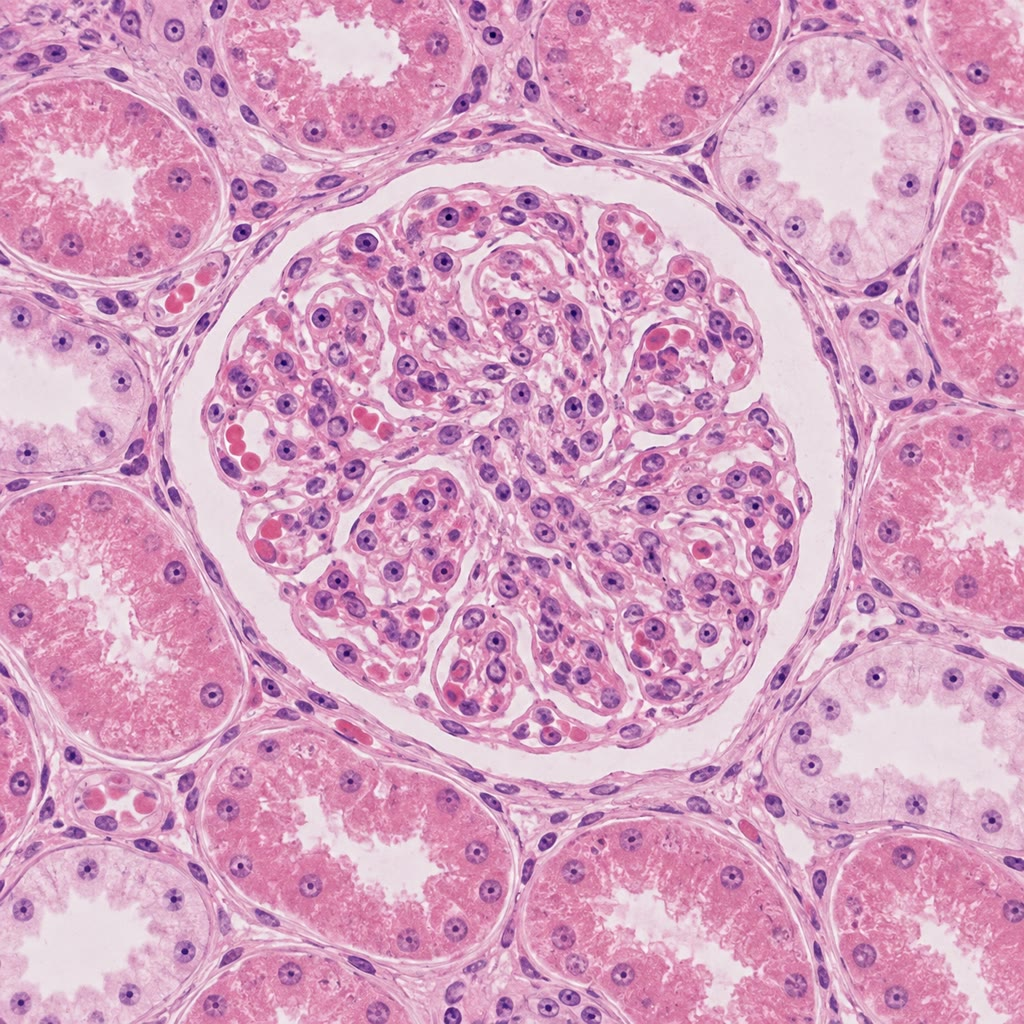
\includegraphics[width=0.46\linewidth]{images/book5/ai/b5-20-kidney-section.jpg}\hspace{0.04\linewidth}
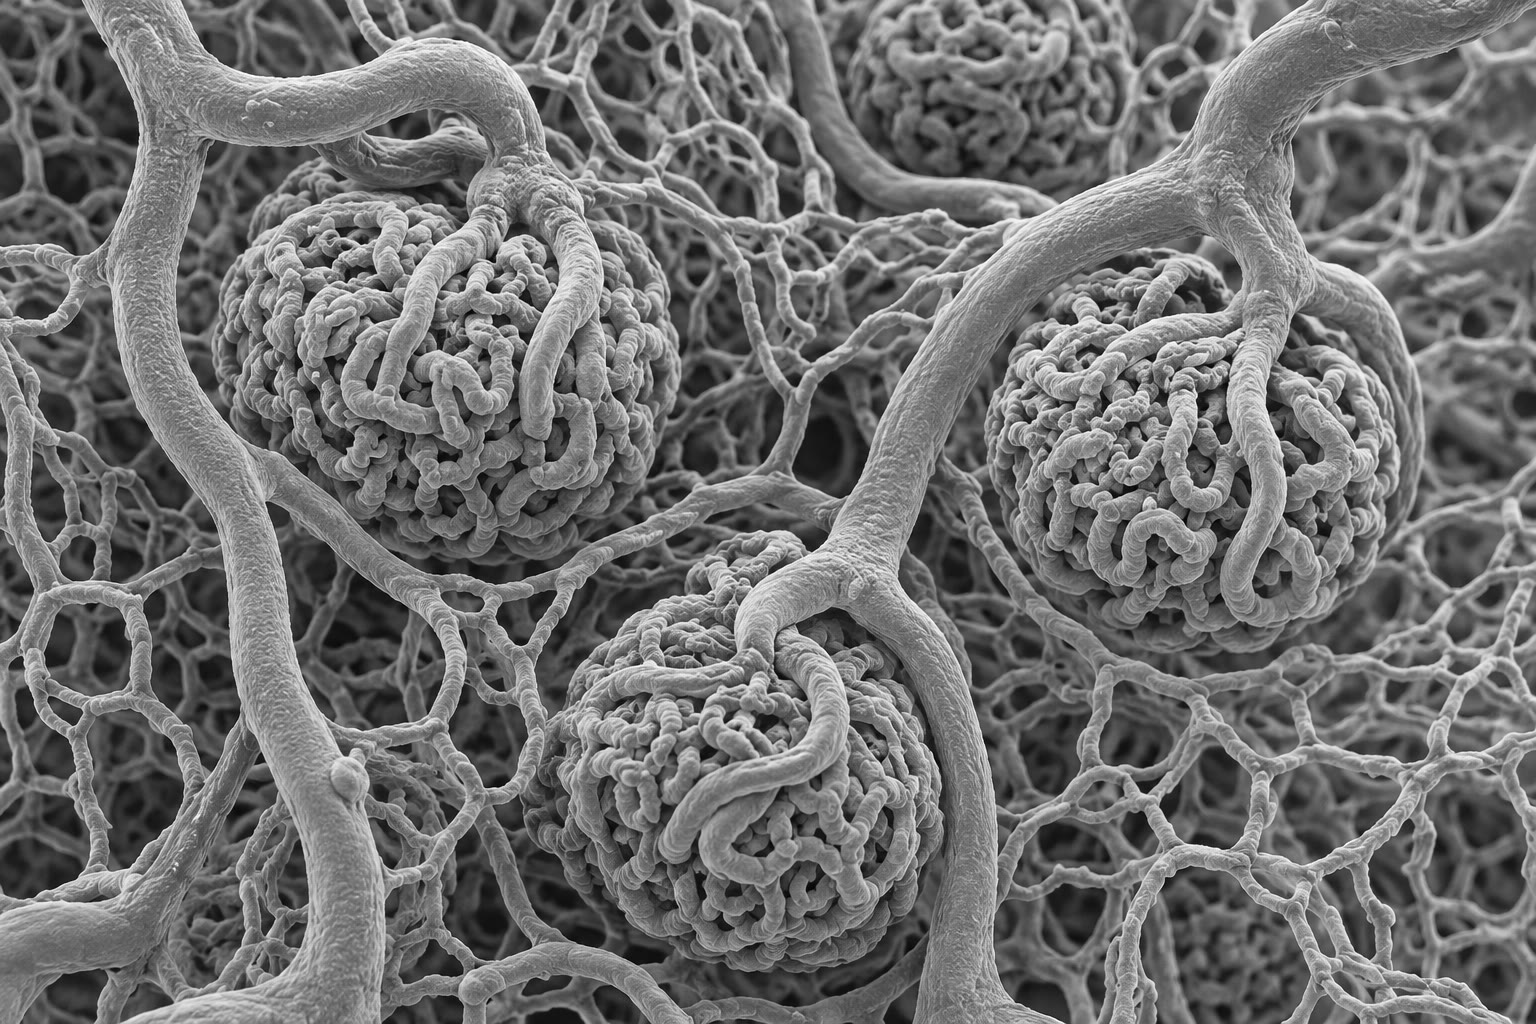
\includegraphics[width=0.46\linewidth]{images/book5/ai/b5-20-nephron-cast.jpg}

{\small يسارًا: قشر الكلية في مقطع --- \omterm{def:b3:renal-osmoregulation:nephron}{كبيبة} في محفظتها بين
مقاطع النبيبات القريبة والبعيدة. ويمينًا: قالب وعائي للقشر،
كل كبّة خيط منه \omterm{def:b3:renal-osmoregulation:nephron}{كبيبة} بوعائيها الوارد والصادر بين الشعيرات
حول النبيبات.}
\end{omfigure}

\section{حيوانات أخرى، وحلول أخرى}

\begin{definition}[تنظيم الأسمولية عبر الحيوانات]\label{def:b3:renal-osmoregulation:comparative}
\index{نبيب مالبيغي}\index{غدة ملحية}\index{خلية كلوريدية}\index{ماء استقلابي}\index{سماكة لبية نسبية}
تعيش أسماك الماء العذب في وسط أسموليته عُشر \omterm{def:b3:renal-osmoregulation:problem}{أسمولية} دمها:
فيندفق الماء داخلًا عبر الخياشيم، ويتسرب الملح خارجًا،
فتطرح بولًا غزيرًا مخففًا وتلتقط الملح التقاطًا فاعلًا عبر
\emph{الخلايا الكلوريدية} في الخياشيم، ولا تشرب أبدًا. وأما
عظميات البحر، ودمها ثلث \omterm{def:b3:renal-osmoregulation:problem}{أسمولية} البحر، فتفقد الماء عبر
الخياشيم، وتشرب ماء البحر، وتضخ الملح خارجًا عبر الخلايا
الكلوريدية نفسها معكوسةً، وتبقي البول شحيحًا؛ وأما القروش
فتبقي دمها متساوي \omterm{def:b3:renal-osmoregulation:problem}{الأسمولية} مع البحر باحتباس البولة (ومعها
أكسيد ثلاثي ميثيل الأمين ليثبّت بروتيناتها في وجهها)، وتطرح
الملح الزائد عبر غدة مستقيمية. وتحمل طيور البحر وزواحفه
\emph{غددًا ملحية} فوق العينين تفرز مُحلولًا ملحيًا أملح من
البحر مرتين، فيقدر القطرس على الشرب من المحيط. وترشّح
الحشرات عبر \emph{نبيبات مالبيغي} التي يسوقها إفراز فاعل
للبوتاسيوم لا ضغط الدم، وتعيد امتصاص الماء في المستقيم إعادةً
تامة حتى يكون رجيع خنفساء صحراوية جافًا. وأما بين الثدييات
فتتدرج قدرة التغليظ مع طول العرى بالنسبة إلى حجم الكلية
(وهي \emph{السماكة اللبية النسبية}): فالقندس يبلغ
\qty{500}{mOsm/L}، والإنسان \num{1200}، والجمل \num{3000}،
وجرذ الكنغر \num{5500} --- وهو ما يتيح له العيش على
\emph{الماء الاستقلابي} المتحرر حين يُؤكسَد غذاؤه، ونحوه
\qty{0.6}{g} من الماء لكل غرام نشاء، بأنف يستعيد الماء من كل
نَفَس زفير بتبريد التيار المعاكس.
\end{definition}

\begin{omfigure}
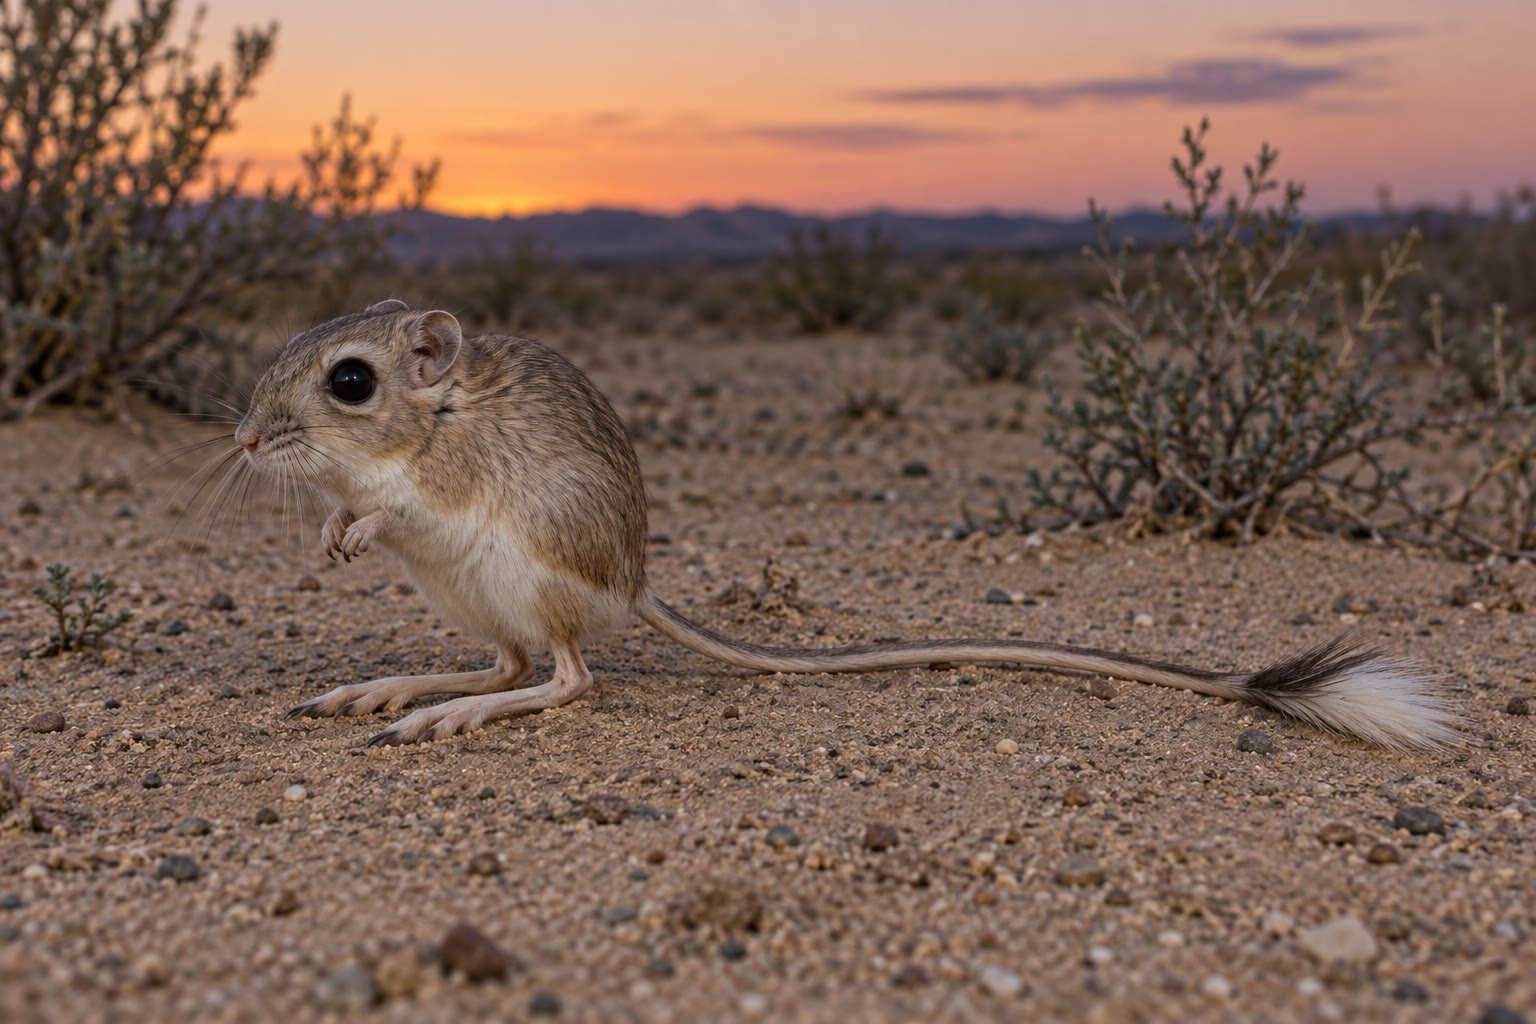
\includegraphics[width=0.56\linewidth]{images/book5/ai/b5-20-kangaroo-rat.jpg}

{\small جرذ كنغر، وهو لا يشرب أبدًا: عرى هنلي طويلة، وبول
أغلظ من ماء البحر خمس مرات، وأنف بارد يكثّف ماء كل نفَس،
وحمية يصنع تأكسدها كل الماء الذي يحتاج إليه.}
\end{omfigure}

\begin{remark}[الكلية مسألةَ تصميم]\label{rem:b3:renal-osmoregulation:design}
ترشّح كلية الثديي أربعين ضعف حجم البلازما في اليوم لتأخذ
ذلك كله راجعًا تقريبًا: وهو تصميم مسرف، مغزاه أن ترشيح كل
شيء وإعادة امتصاصه انتقائيًا أبسط من إفراز كل فضلة قد تظهر
إفرازًا انتقائيًا. وكلفته \qty{7}{\%} من استقلاب الراحة
تُنفَق في ضخ الصوديوم راجعًا، ومكمن ضعفه المرشِّح الرقيق،
الذي يخفق ببطء تحت الضغط العالي والغلوكوز العالي. وأما
براعته فعروة التيار المعاكس، وهي أداة توجد أيضًا في مثانات
سباحة أسماك العمق، وفي سيقان الطيور الخائضة، وفي أنوف قوارض
الصحراء، يُكدَّس بها فرق موضعي صغير محتمَل في فرق كبير ---
وهي في كل حالة الفكرة نفسها: أن التدرج يمكن أن يُبنى من
الجريان.
\end{remark}

\section{تمارين}

\begin{exercise}[$\star$]\label{exo:b3:renal-osmoregulation:1}
سمّ قطع \omterm{def:b3:renal-osmoregulation:nephron}{النفرون} بالترتيب واذكر شيئًا واحدًا تفعله كل قطعة.
\end{exercise}

\begin{exercise}[$\star$]\label{exo:b3:renal-osmoregulation:2}
عرّف التصفية. مادة تركيزها في البلازما \qty{2}{mg/mL}، وفي
البول \qty{100}{mg/mL}، وجريان البول \qty{1.5}{mL/min}. احسب
تصفيتها وقل هل تُعاد امتصاصها أم تُفرَز أم لا هذا ولا ذاك،
إذا كان معدل الرشح \qty{120}{mL/min}.
\end{exercise}

\begin{exercise}[$\star$]\label{exo:b3:renal-osmoregulation:3}
لماذا لا تشرب سمكة الماء العذب أبدًا وتشرب سمكة البحر
باستمرار؟ وماذا تفعل الخياشيم في كل منهما؟
\end{exercise}

\begin{exercise}[$\star$]\label{exo:b3:renal-osmoregulation:4}
ما \omterm{prop:b3:renal-osmoregulation:countercurrent}{الأثر المفرد} في \omterm{def:b3:renal-osmoregulation:nephron}{عروة هنلي}، وأي فرع ينتجه، ولماذا يجب أن
يختلف الفرعان في نفوذيتهما للماء؟
\end{exercise}

\begin{exercise}[$\star\star$]\label{exo:b3:renal-osmoregulation:5}
ضغط الشعيرة الكبيبية \qty{60}{mmHg}، وحيز بومان
\qty{18}{mmHg}، والضغط الجرمي للبلازما \qty{28}{mmHg} عند
الطرف الوارد مرتفعًا إلى \qty{35}{mmHg} عند الطرف الصادر.
احسب ضغط الرشح الصافي عند كل طرف واشرح لماذا قد يتوقف الرشح
قبل نهاية الشعيرة. وماذا يقتضي ذلك في أثر الجريان البلازمي
على معدل الرشح؟
\end{exercise}

\begin{exercise}[$\star\star$]\label{exo:b3:renal-osmoregulation:6}
تصفية الكرياتينين عند مريض \qty{40}{mL/min}. وصوديوم البلازما
\qty{140}{mmol/L}، وصوديوم البول \qty{70}{mmol/L}، وجريان البول
\qty{1}{mL/min}. احسب الحمل المرشَّح من الصوديوم، والطرح،
والنسبة المعاد امتصاصها، وتصفية الصوديوم.
\end{exercise}

\begin{exercise}[$\star\star$]\label{exo:b3:renal-osmoregulation:7}
شخص يتناول حميةً تنتج \qty{900}{mOsm} من المذاب في اليوم ويقدر
على التغليظ إلى \qty{1200}{mOsm/L}. فما أدنى حجم بول؟ وإذا خفض
داء كلوي الأقصى إلى \qty{400}{mOsm/L}، فكم يجب أن يشرب ليبقى
في توازن، مع حساب \qty{0.9}{L} من الفقد غير المحسوس؟
\end{exercise}

\begin{exercise}[$\star\star$]\label{exo:b3:renal-osmoregulation:8}
تنبأ بحجم البول وأسموليته، وبصوديوم البلازما، وبحال العطش في
(أ) البيلة التفهة، و(ب) إفراز غير ملائم للفازوبريسين من \omterm{def:b3:cancer-biology:hallmarks}{ورم}،
و(ج) فرط \omterm{def:b3:renal-osmoregulation:controls}{الألدوستيرون}، و(د) حمية بلا ملح أسبوعًا.
\end{exercise}

\begin{exercise}[$\star\star$]\label{exo:b3:renal-osmoregulation:9}
احسب \omterm{prop:b3:renal-osmoregulation:water}{تصفية الماء الحر} لبول عند \qty{100}{mOsm/L} بجريان
\qty{6}{mL/min} ولبول عند \qty{1000}{mOsm/L} بجريان
\qty{0.6}{mL/min}، والبلازما عند \qty{300}{mOsm/L}. وفسّر كلًّا منهما.
\end{exercise}

\begin{exercise}[$\star\star\star$]\label{exo:b3:renal-osmoregulation:10}
نمذج العروة $n$ مرحلةً يكون فيها السائل الصاعد عند كل مرحلة
دون الخلال بمقدار \qty{200}{mOsm/L} ويساويه السائل النازل، والسائل
الداخل عند \qty{300}{mOsm/L}. واحتجّ لأن \omterm{def:b3:renal-osmoregulation:problem}{أسمولية} الحالة
المستقرة عند المنعطف تقدر على أن تقارب $300 +
200n$، فيكون التدرج محدودًا بطول العروة وبالأثر المفرد
للمضخة، وقل ما الذي يحدد $n$ فيزيائيًا.
\end{exercise}

\begin{exercise}[$\star\star\star$]\label{exo:b3:renal-osmoregulation:11}
يأكل جرذ الكنغر \qty{5}{g} من البذر الجاف في اليوم،
\qty{80}{\%} منها نشاء، تُؤكسَد إلى CO$_{2}$ وماء (\qty{0.6}{g}
ماء لكل غرام نشاء). وعليه أن يطرح \qty{3}{mOsm} من المذاب في
اليوم عند \qty{5500}{mOsm/L}، ويفقد \qty{1.5}{g} من الماء في
اليوم تبخرًا من أنف يستعيد \qty{70}{\%} من ماء نفَسه. وازِن
ميزانيته المائية وقل هل ينجو من غير أن يشرب.
\end{exercise}

\begin{exercise}[$\star\star\star$]\label{exo:b3:renal-osmoregulation:12}
يمرر الديال الدمَ على جانب من غشاء والسائل الديالي على
الجانب الآخر، في تيار معاكس. اشرح لماذا يصفّي الجريان
المعاكس أكثر من الجريان المتوازي، وقدّر تصفية آلة تزيل
البولة من \qty{300}{mL/min} من الدم بكفاءة \qty{70}{\%}،
وقارن ذلك بكليتين على مدى أسبوع إذا عملت الآلة أربع ساعات
ثلاث مرات في الأسبوع.
\end{exercise}

\section{مسألة: ثمانية عشر دلوًا في اليوم}

\begin{problem}[{مسألة نهاية الأسبوع --- راشح يوم يُتبَّع من
الكبيبة إلى المثانة: ضغوط ستارلنغ، وتصفيات أربع مواد، وعتبة
الغلوكوز، وميزانية الماء من أقصى تخفيف إلى ماء البحر، وميزان
قارض صحراوي، وتُختم بمعدل الرشح، وبحجم البول الإجباري،
وبصافي الماء الذي يعطيه لتر من ماء البحر}]
\label{pb:b3:renal-osmoregulation:1}
المعطيات: $K_{f} = \qty{12.5}{mL/min/mmHg}$؛ و$P_{\text{GC}} = \qty{55}{mmHg}$،
و$P_{\text{BS}} = \qty{15}{mmHg}$، و$\pi_{\text{GC}} = \qty{30}{mmHg}$.
والبلازما: إنولين \qty{0.5}{mg/mL}، وكرياتينين \qty{0.01}{mg/mL}،
وبولة \qty{5}{mmol/L}، وغلوكوز \qty{5}{mmol/L}، وبارا-أمينوهيبورات
\qty{0.02}{mg/mL}، وNa$^{+}$ \qty{140}{mmol/L}، \omterm{def:b3:renal-osmoregulation:problem}{وأسمولية}
\qty{290}{mOsm/L}. وجريان البول \qty{1}{mL/min}: إنولين \qty{62.5}{mg/mL}،
وكرياتينين \qty{1.3}{mg/mL}، وبولة \qty{250}{mmol/L}، وغلوكوز $0$،
وبارا-أمينوهيبورات \qty{13}{mg/mL}، وNa$^{+}$ \qty{100}{mmol/L}،
\omterm{def:b3:renal-osmoregulation:problem}{وأسمولية} \qty{600}{mOsm/L}. والمكداس $0.45$. وللغلوكوز $T_{m} =
\qty{375}{mg/min}$ (\qty{2.1}{mmol/min}). والمذاب اليومي \qty{600}{mOsm}؛
و$U_{\max} = \qty{1200}{mOsm/L}$، و$U_{\min} = \qty{50}{mOsm/L}$؛
والفقد غير المحسوس \qty{0.9}{L/d}؛ وماء البحر \qty{1000}{mOsm/L}.

\medskip
\noindent\textbf{الجزء الأول --- المرشِّح.}
\begin{enumerate}
  \item احسب ضغط الرشح الصافي \omterm{thm:b3:renal-osmoregulation:clearance}{ومعدل الرشح الكبيبي}.
  \item حوّل معدل الرشح إلى لترات في اليوم. وكم مرة يُرشَّح حجم
        البلازما (\qty{3}{L})؟
  \item احسب تصفية الإنولين وقارنها بمعدل الرشح. واحسب تصفية
        الكرياتينين؛ ولماذا تكون أكبر قليلًا؟
  \item احسب تصفية البارا-أمينوهيبورات (وهي الجريان البلازمي
        الكلوي)، والجريان الدموي الكلوي، ونسبة الرشح.
  \item ينقبض الشُّرين الصادر فيرفع $P_{\text{GC}}$ إلى
        \qty{60}{mmHg}. فما معدل الرشح الجديد؟ ولماذا تخفض
        الأدوية الحاجبة للأنجيوتنسين II معدل الرشح قليلًا في
        كلية سليمة وتحمي كلية سكرية؟
  \item يظهر البروتين في البول عند \qty{3}{g/d}. فأي طبقة من
        المرشِّح أخفقت، وماذا يحدث للضغط الجرمي في البلازما
        وللنسج إن استمر ذلك؟
\end{enumerate}

\medskip
\noindent\textbf{الجزء الثاني --- المعالجة.}
\begin{enumerate}[resume]
  \item البولة: الحمل المرشَّح، والطرح، والنسبة المعاد
        امتصاصها، والتصفية.
  \item الصوديوم: الحمل المرشَّح في اليوم بالمولات وبالغرامات،
        والطرح، والنسبة المعاد امتصاصها. وكم كيلوغرامًا من
        الملح كان سيُفقد في اليوم لو لم يُعَد امتصاص شيء؟
  \item الغلوكوز: الحمل المرشَّح بالميلي مول في الدقيقة وبالغرامات في
        اليوم؛ وهل يُطرح منه شيء؟ وعند أي غلوكوز بلازمي يبلغ
        الحمل المرشَّح $T_{m}$ (العتبة)؟
  \item غلوكوز البلازما عند مريض سكري \qty{20}{mmol/L}. احسب
        الغلوكوز المطروح في الدقيقة وفي اليوم بالغرامات، وحجم
        البول الإضافي إذا حمل كل \qty{300}{mOsm} من الغلوكوز
        \qty{1}{L} عند التركيز السائد. واشرح عطش السكري غير
        المعالج ونقص وزنه.
  \item تكلف إعادة امتصاص الصوديوم ATP واحدًا لكل ثلاثة
        Na$^{+}$. فكم مولًا من ATP تنفق الكلية على الصوديوم في
        اليوم، وكم كيلوجول ذلك (\qty{50}{kJ/mol})؟ وقارن ذلك
        باستقلاب راحة قدره \qty{7}{MJ/d}.
  \item اشرح لماذا ترشّح الكلية وتعيد الامتصاص بدل أن تفرز كل
        فضلة، من حيث ما سيلزم النبيبَ أن يتعرفه.
\end{enumerate}

\medskip
\noindent\textbf{الجزء الثالث --- الماء.}
\begin{enumerate}[resume]
  \item التصفية \omterm{def:b3:renal-osmoregulation:problem}{الأسمولية} $U_{\text{osm}}V/P_{\text{osm}}$ من
        المعطيات، \omterm{prop:b3:renal-osmoregulation:water}{وتصفية الماء الحر}. فهل الشخص يحفظ الماء أم
        يطرحه؟
  \item أدنى حجم بول للمذاب اليومي؛ وأقصاه (عند $U_{\min}$)؛
        ومجموع الحاجة اليومية للماء عند الأدنى، مع الفقد غير
        المحسوس.
  \item يُشرب لتر من ماء البحر. فكم بولًا يلزم لطرح ملحه عند
        $U_{\max}$، وما صافي الكسب المائي قبل حساب مذاب اليوم
        نفسه؟ وبعده؟
  \item الفازوبريسين غائب (بيلة تفهة) ويبقى البول عند
        $U_{\min}$. فما حجم البول اليومي للمذاب نفسه، وكم ماءً
        يجب أن يُشرب كل يوم للبقاء في توازن؟
  \item جعة عند \qty{20}{mOsm/L}: كم يمكن أن يُشرب منها في
        اليوم قبل أن تعجز الكلية، عند $U_{\min}$، عن طرح
        الماء؟ (فالماء الزائد على ما يقدر المذاب على حمله عند
        $U_{\min}$ يتراكم.)
  \item بعد ليلة بلا ماء تكون \omterm{def:b3:renal-osmoregulation:problem}{أسمولية} البلازما \qty{298}{mOsm/L}.
        فبأي نسبة مئوية ارتفعت، وماذا يفعل الوطاء؟ وقدّر
        العجز المائي إذا كان مجموع ماء الجسم \qty{42}{L}
        والمذاب بلا تغيّر.
  \item اشرح لماذا قد يصاب عدّاء ماراثون يشرب \qty{6}{L} من
        الماء وهو يعرق ملحًا بصوديوم بلازمي منخفض خطرًا، وما
        الذي كان على الكلية أن تفعله لتمنع ذلك.
\end{enumerate}

\medskip
\noindent\textbf{الجزء الرابع --- الصحراء.}
\begin{enumerate}[resume]
  \item يطرح جرذ الكنغر \qty{3}{mOsm} في اليوم عند \qty{5500}{mOsm/L}.
        فما حجم البول؟ وقارن ذلك بالحجم الذي كانت ستحتاج إليه
        كلية بشرية للمذاب نفسه عند أقصاها هي.
  \item يعطي غذاؤه \qty{2.4}{g} من \omterm{def:b3:renal-osmoregulation:comparative}{الماء الاستقلابي} في اليوم
        ويفقد \qty{1.6}{g} بالتنفس و\qty{0.3}{g} في الرجيع.
        وازِن الميزانية مع بول السؤال 20.
  \item جمل يغلّظ إلى \qty{3000}{mOsm/L} ويحتمل فقد \qty{25}{\%}
        من ماء جسمه. فلجمل كتلته \qty{500}{kg} وماؤه
        \qty{65}{\%}، كم يقدر على أن يفقد، وكم يومًا يغطي ذلك
        عند فقد قدره \qty{5}{L/d}؟
  \item طائر بحري يأكل \qty{200}{g} من السمك ويشرب \qty{100}{mL}
        من ماء البحر في اليوم، فيدخل \qty{150}{mmol} من NaCl.
        وغدته الملحية تفرز عند \qty{800}{mmol/L}. فكم محلولًا
        ملحيًا ينتج، ولماذا تكون الغدة أفضل من الكلية (التي
        تغلّظ في الطيور إلى \qty{600}{mOsm/L} فقط) في هذا؟
  \item سمكة ماء عذب كتلتها \qty{100}{g} تكسب \qty{30}{\%} من
        كتلة جسمها ماءً في اليوم عبر خياشيمها. فكم بولًا يجب أن
        تصنع، وعند أي \omterm{def:b3:renal-osmoregulation:problem}{أسمولية} بالنسبة إلى دمها، وماذا كان
        سيحدث لملحها بلا التقاط فاعل؟
  \item لخّص: \omterm{thm:b3:renal-osmoregulation:clearance}{معدل الرشح الكبيبي} (السؤال~1)، وحجم البول
        الإجباري (السؤال~14)، وصافي الماء من لتر من ماء البحر
        بعد حساب مذاب اليوم (السؤال~15).
\end{enumerate}
\end{problem}
